\clearpage
\item \subquestionpoints{3} \textbf{Coding problem.}
In \texttt{src/p01e\_gda.py}, fill in the code to
calculate $\phi$, $\mu_{0}$, $\mu_{1}$, and $\Sigma$, use these parameters
to derive $\theta$, and use the resulting GDA model to make predictions on the
validation set.

\ifnum\solutions=1 {
  \begin{answer}
\newline
  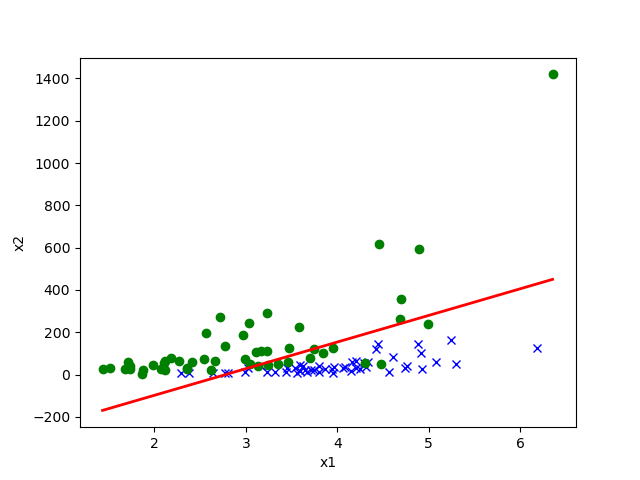
\includegraphics[height=5.5cm]{C:/Users/feroc/OneDrive/Notability/CS229 Machine Learning/problem_sets/ps1/src/output/p01e_pred_1.png}
  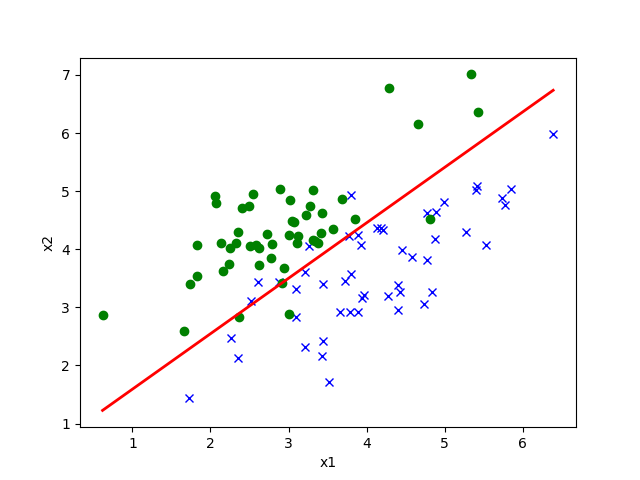
\includegraphics[height=5.5cm]{C:/Users/feroc/OneDrive/Notability/CS229 Machine Learning/problem_sets/ps1/src/output/p01e_pred_2.png}
\end{answer}

} \fi
